\section{Background}


Since the dawn of the 21st century, the era of 'Big Data' is shaping the way people live, learn and entertain. 
The need to handle the exponentially generated and accumulated data from varied sources like mobile devices, mechanical sensors, financial transactions,
satellite imaging makes the task of data managing more and more challenging
day after day. 
With the usage of digital gadgets and industrial machinery presents a rapid increase, the amount of data generated reaches an astonishing level that is far higher than ever in history. 
According to a fact sheet organized by Mark Mulcahy \cite{factsheet} from Waterford Technologies, 2.7 Zetabytes of data exist in the digital world today, in which social media platforms like Facebook stores, accesses, and analyzes 30+ Petabytes of user generated data; search engines like Google was processing 20,000 terabytes of data (20 petabytes) a day; retail industries like Walmart handles more than 1 million customer transactions every hour. \\

\noindent Besides the volume of data, the collected raw data are in a wide range of
formats, most are unstructured, like images, videos, audios, etc. The proliferation of social media platform is the main contributor to such rapid generation of data, which records the implicit pattern of the activities and habits of the individuals or the entities who generated the data in an exponentially increasing rate. Therefore massive data mining for customer profiling and user clustering to pinpoint the marketing campaign towards the target group has become a popular pursuit in business intelligence analytics for optimization of cost controlling. In order to ensure the feasibility and efficiency of the real-time analysis of constantly in-coming raw data, or carry out user behavior pattern mining from tons of historical data, the databases for storage have to keep up with the requirements proposed by the marketplace nowadays. The consistency,
accessibility, velocity of data inserting and retrieving might make a
huge difference in data manipulation tasks, especially in
fields like finance, social networks, etc, thus making optimal choices
of the right databases for different data formats, different data volume,
different business focuses plays a very
important part in the whole data processing pipeline.



\section{Introduction of NoSQL Databases}

NoSQL, for "Not Only SQL", and as summarized by Moniruzzaman and Akhter Hossain\cite{DBLP:journals/corr/MoniruzzamanH13}, it refers to distributed and non-relational data management systems designed for large-scale data
storage and for massively-parallel data processing across a large number of commodity
servers. Unlike its conventional RDBMS counterparts which display the relation embedded in the dataset in the format of tables, on which impose a strictly constrained schema to ensure the homogeneity of data entries in each columns (or attributes), NoSQL breaks the rule of pre-defining schema and stores the dataset in the semi-structured json format, which makes it more practical when used for temporary caching of incoming raw data, especially unstructured raw data. Its schemaless design fits in most real-life data mining cases in industry since it is a normal scenario to collect un-cleaned and messy first-hand raw data without shared resemblance in structure from the users, who come from varied fields of professions. Hence the ability to process massive amount of data with a schema-less structure is what makes NoSQL more popular in data mining industries where the data that most engineers and data scientists have to work with are  unstructured with flexible schema.
The architecture of NoSQL databases are distributed and fault-tolerant by utilizing replica sets among multiple machine to 
guarantee data availability in the case of network disruption or when certain servers accidentally go down.
To reach a
balance between availability and consistency, NoSQL preserves a higher
level of consistency by slightly sacrificing its availability.  \\


\noindent In a way, RDBMS is still the mainstay in industry because it has been around for a longer period of time and it is widely applied in industry and academic work when the web space has not seen such rampant digital gadgets proliferation and rapid data generation, so it is not built to support distributed system in the first place. With limited amount of data to manipulate, the consistency as well as referential integrity become essential tasks to be guaranteed. But it is exactly the strong focus of relational DBMS on ensuring ACID \cite{Schram2012MySQLTN} (Atomicity, Consistency, Isolation and
Durability) that makes it difficult for scaling, which is one of
the many reasons why most companies from giant enterprises to startups are considering migrating their partial or even entire database from RDBMS to NoSQL as business expands. \\

\noindent NoSQL is not built for the entire replacement of SQL, but as a complementary option depending on different tasks. Trade-offs have to be made because once the data are segmented and scattered across multiple clusters for storage and parallel processing, immediate up-to-date consistency is broken due to  unavoidable latency across the entire network. To handle huge volume of high-dimensional data, the urgent demand is the capacity and flexibility of the database, which calls for the priority to be put to the scalability of the database system.
  With sharding, which would be explored in more details later, it partitions data onto a cluster of remote machines, boosting the overall performance while controlling cost with cheap commodity hardware. 
  
  
\begin{figure}[H]
	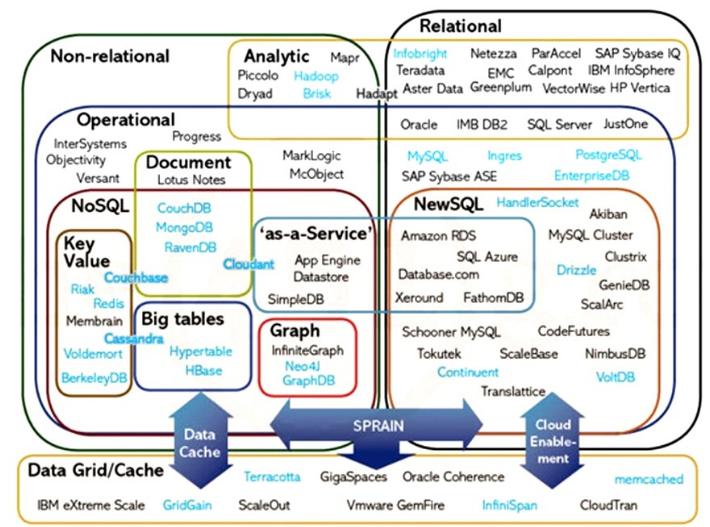
\includegraphics[height=7cm, width=9cm]{../../../images/nosql.png}
	\caption{NoSQL Databases In Industries (Source: \cite{DBLP:journals/corr/MoniruzzamanH13})}
\end{figure}

  
\noindent To take fully advantage of its features such as flexible schema, server failure tolerance and  horizontally scalability by cheap commodity hardware, primary uses of NoSQL Database mainly focus on tasks that requires high velocity of data transaction to guarantee consistency among multiple machines as well as capacity for massive data storage to assure availability. And according to Moniruzzaman and Akhter Hossain\cite{DBLP:journals/corr/MoniruzzamanH13}, these uses include 
\begin{itemize}
\item (1) Large-scale data processing (parallel
 processing over distributed systems); 
 \item (2) Embedded IR (basic machine-to-machine
 information look-up \& retrieval); 
 \item (3) Exploratory analytics on semi-structured data (expert
 level); 
 \item (4) Large volume data storage (unstructured, semi-structured, small-packet structured).
\end{itemize}

\[\]
\section{Characteristics of NoSQL Databases}



\subsection{Availability}

\subsubsection{Replication}\mbox{}

\noindent To guarantee high availability, the mechanism of failover is utilized by creating replica sets as remedy for server malfunctions, network disruptions, system maintenance and upgrade. In the distributed system that is horizontally scaled, consistency is no longer satisfied. Therefore with latency exists in the process of data collection, replica generation is also asynchronous. Without requiring manual setup to create replica of data chunks across cluster after reading in data each time, the  replication function is embedded in th NoSQL DBMS as one of its major features and automatically triggered to prepare for any unexpected server failure. 

\subsection{Scalability}


\subsubsection{Sharding}\mbox{}


\noindent Sharding is a method for distributing data across multiple machines to scale the system horizontally by adding more servers to divide the overall workload, hence increase capacity to support deployment of applications that require manipulation of large data sets or high throughput operations. However the improvement of performance comes with sacrifice as well. Across partitions, operations such as joins are not feasible since the lack of consistency and flexible schema all violate the prerequisite of executing joins. Complex relation features are not supported and referential integrity constraints can also no longer be maintained. \\

\noindent In the partitioning step, there are mainly 2 sharding strategies. One is hashed sharding, which computes the hash value of the shard keys using carefully designed hash functions to distribute the data as balanced as possible to multiple workers on a cluster to process in parallel and the other is ranged sharding that divides data into ranges based on the shard keys, so that the more similar shard keys are more likely to be assigned to the same chunk. But with ranged sharding, efficiency heavily depends on the shard keys chosen. Wrong choices might result in uneven distribution of data, therefore causing performance bottlenecks. 


\subsection{Consistency}\mbox{}

\noindent As a distributed system, since the writes of data into storage is asynchronous, thus with different architecture, the real-time consistency is not guaranteed, which indicates that clients from different regions are not able to retrieve the same version of data at the same time. But the eventual consistency is absolute after all updates are propagated throughout the system.

\subsubsection{Master-slave}\mbox{}

\noindent For databases with a master-slave mechanism, all writes into the database are written to the master node, and all reads are processed through the replication set of slave nodes. This centralization architecture could encounter significant inconvenience when the incoming dataset is large, the step when the master node receives the data and then passes them down to slave nodes for duplication and backup will slow down the entire processing speed. Moreover, if the data written in is somehow incorrect, the mistake would be propagated down to all the slave nodes as well, hence providing the wrong version of data to the users for that the master node is the only source that receives the input raw data.

\subsubsection{Peer-to-peer}\mbox{}

\noindent A peer-to-peer architecture is considered a decentralized system where there exists no hierarchical order with a master controlling the overwriting and permission-granting power for data nodes intercommunication. Each node of the cluster is identical to other nodes in the same cluster and all nodes follow the dissemination membership protocol \cite{DBLP:journals/corr/abs-1712-04344} and could be considered as request coordinators. Unlike master-slave structure, with peer-to-peer system, the instant consistency could be assured since in the system, not only do peers have the permission of reading operation, but they are also eligible for receiving data from the clients' end and writing into database for immediate backup. Under this mechanism, real-time update of each node in the cluster is shared across the system with other peers. Besides playing the role as the receiver, when the database is requested by queries from users to provide chunks of data they expect, the actions among peers are determined by co-ordination since there is no longer a higher-ranking node responsible for dividing and delegating jobs for workers to finish in parallel. One of the NoSQL DBMS used in industry that adopts peer-to-peer distributed
architecture is Cassandra:

\begin{figure}[H]
	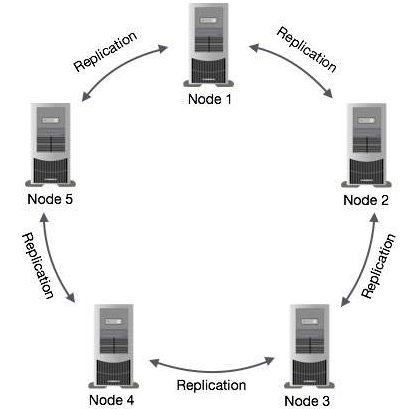
\includegraphics[height=7cm, width=8cm]{../../../images/casa.png}
	\caption{Cassandra Peer to Peer Architecture (Source: \cite{DBLP:journals/corr/abs-1712-04344})}
\end{figure}




\subsection{Summary}
To summarize, since all these three characteristics (Availability, Scalability and Consistency) can not be simultaneously achieved according to CAP theorem \cite{Brewer2012CAPTY}, 

\begin{figure}[H]
	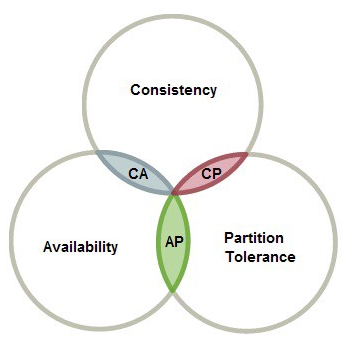
\includegraphics[height=7cm, width=8cm]{../../../images/cap.png}
	\caption{CAP Theorem (Source: \cite{Brewer2012CAPTY})}
\end{figure}

\noindent thus compromises are made for trade-offs and balance is reached with the BASE theorem \cite{Brewer2012CAPTY}(Basically Available, Soft-state, Eventually consistent).

\[\]

\section{Data Models of NoSQL Databases}

 In order to cater to the velocity demand for processing and the variety of the data format generated from different sources depending on the different products and services each company offers to their target clients, NoSQL DBMS currently used in industries are divided into four categories, among each  there are several major database systems that are most widely used: Redis as key-value store database, HBase as column-oriented database, MongoDB as document-oriented database and Neo4j as graph database.

\subsection{Key-Value Databases}

Key-value databases has been around for decades and it's popular among users for its common data structure (key value pair) to store data is easy to understand for java and python programmers because key-value pair shares resemblance with HashMap class in java as well as Dictionary class in python. In key-value databases, keys as field names, are normally represented as unique alpha-numeric identifiers and converted to hashes for more efficient search and retrieve. Correspondingly, the content stored under this field name is its value, which supports various formats of data such as sets, strings and lists. Together, keys and values are stored in standalone hash tables. The performance of key-value databases are mainly affected by:


\begin{itemize}
	\item the design of the hashing function applied to keys. A good hashing function results in fewer conflicts, which ends up with evenly distributed data across all slots;
	\item the size and data format of the corresponding value stored, if the volume of values under each key exceed a certain constraint, then the process of writing into and retrieving from the table could be significantly slowed down, thus compromising the efficiency of the entire task;
\end{itemize}

\noindent Since consistency is guaranteed only for operations on a single key, so it would not be an optimal choice for multi-operation transactions or for tasks that involve complex relationship among attributes. However, its simple data structure and compatibility to support multiple data formats assures its outstanding velocity of data processing compared with other  NoSQL databases, thus key-value databases are preferred for caching, user profile managing or shopping cart retrieval. This is why Amazon makes extensive use of its own key value system called Dynamo \cite{DBLP:journals/corr/MoniruzzamanH13}, a highly available key-value storage
system that provides highly available and scalable
distributed data store in its shopping cart. 

\subsubsection{Redis}\mbox{}\mbox{}

\noindent As a NoSQL database written in C++, the excel performance and high I/O speed of Redis makes it an optimal choice for 
caching. Redis supports varied data structures such as list, queue, set (basic operations like union, intersection, difference), hash table, stc. 
Redis is preferred for applications with real-time data collecting and processing, which specifically requires high I/O speed because the incoming data is updating rapidly.

\subsection{Column-oriented Databases}

An en extension to the key-value pair storage mechanism, column-oriented database storage system places the attributes (keys) as headers, and serialized corresponding values normally with high dimensions and homogeneous as a column in each data entry. It could be considered as a transposition of row-based storage strategy for the benefit of lowering the overhead when traversing the whole row-based table to extract the information requested by the query from users. 


\subsubsection{HBase}\mbox{}\mbox{}

\noindent As a distributed data storage system, HBase is specifically designed for processing and storing data with massive volume and sparsity, by adopting Hadoop Distributed File System (HDFS) \cite{Vora2011HadoopHBaseFL}
underneath. It provides similar functions as BigTable \cite{Chang2006BigtableAD}, from which the design of HBase is inspired. What makes it special from the other NoSQL database systems is that besides supporting  the storage of massive amount of data, it also provides unparalleled advantage in the analytic and pattern mining using MapReduce and Spark  without incurring extra overhead cost by migrating the data, because HBase is already part of the Apache Hadoop ecosystem. Hence the support of data manipulation pipeline is seamless.

\subsection{Document-oriented Databases}

Unlike RDBMS designed to store data as tables, Document-oriented Databases are designed to store documents encoded in semi-structured standard \cite{DBLP:journals/corr/MoniruzzamanH13} data exchange
format such as XML, JSON (Javascript Option Notation) or BSON (Binary JSON).

\begin{figure}[H]
	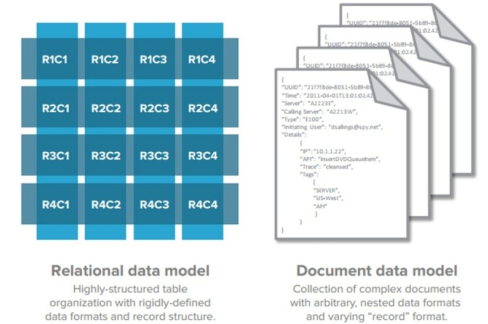
\includegraphics[height=6cm, width=8cm]{../../../images/vs.png}
	\caption{Relational data model vs. Document data model (Source: \cite{DBLP:journals/corr/MoniruzzamanH13})}
\end{figure}


 \noindent Due to its schema-free feature, under each attribute, multiple nested sub-attributes could be stored in flexible structures that do not have to be identical to each other, which makes Document-oriented databases the perfect option for storing irregular and  sparse data. Because if the amount of missing values is significant in RDBMS, to guarantee a fixed schema structure for the table format, all the missing data would be filled by nulls as placeholders. And in this case, excessive memory would be wasted for unnecessary storage.  


\subsubsection{MongoDB}\mbox{}

 \noindent Among many NoSQL databases, MongoDB is considered the most popular with the largest number of users. Because not only does it has features of NoSQL database system like flexible schema, easy to scale out and also MongoDB is quite SQL-friendly, for instance, MongoDB allows users to create indexes to speed up the searching process. And the support of writing quries in Javascript and inserting data with a semi-structured format like json, bson, etc. makes MongoDB a user-friendly choice because unlike the other NoSQL databases, it does not require users to learn new syntax specific to the database in order to start using it.


\subsection{Graph Databases}\mbox{}

\noindent Graph databases replace relational tables with structured relational graphs of
interconnected key-value pairings\cite{DBLP:journals/corr/MoniruzzamanH13}. Graph theory is applied to the storage of data in graph-based databases, in which each node represents an attribute while each edge represents a relationship between two adjacent nodes, making it nearly as powerful as relational databases when it comes to dataset with complicated relations such as social network. For graph-based databases, it is easy to model all relations that are supported in RDBMS, such as one-to-one, one-to-many and many-to-many because of its hyper-relational feature. But as an improvement compared with relational databases when executing join across multiple tables, graph-based databases aggregate different tables with a much more readable relationship identifier to query data using Depth First Search or Breadth First Search, indicating the fact that it is most suitable for dataset in hierarchical tree structures. Hence it's widely used to map out relationships on social networks and make recommendations for e-commerce platforms.


\subsubsection{Neo4J}\mbox{}

\noindent Neo4J is a graph database that is currently under development. With full ACID \cite{Schram2012MySQLTN} (Atomicity, Consistency, Isolation and
Durability) support, it is capable of providing highly availability and stability. It uses a querying language called Cypher \cite{Webber2012API}, a declarative language, to execute searching and matching. Both unidirectional and bidirectional relations are supported in Neo4J, which is distinguished by the use of a dotted line in Cypher either with or without an arrow at the end of the line.

\[\]
\section{Benefits And Drawbacks}

\subsection{Benefits}

\subsubsection{Scaling Capability}\mbox{}


\noindent Due to the fact that the rapid expansion and generation of data pushes the conventional RDBMS to its limit and calls for a data storage system to cater to the exponentially increasing demand,  industries are seeking more efficient databases like NoSQL to migrate and storage their data.
Using sharding to partition data onto a cluster of remote machines, NoSQL boosts the overall performance while controlling cost with cheap commodity hardware.


\subsubsection{Flexible schema} \mbox{}

\noindent Compared with the conventional RDBMS that any changes of schema must be carefully managed, NoSQL databases has more flexible structure of data and do not need extra adjustments when there are additional requests to update the original schema. 


\subsubsection{Cost}\mbox{}

\noindent One outstanding feature that makes NoSQL a widely used database among various industries with massive amount of data manipulation involved is that it takes advantage of clusters of cheap commodity servers for data storage and transaction.
Compared with expensive propriety servers that RDBMS used to rely on, cost per transaction using NoSQL is lower, so NoSQL is considered much more economically preferable.  


\subsection{Drawbacks}

However there are still many remaining problems which NoSQL
databases cannot solve:

\subsubsection{Not Support Complex  Relationships or ACID Transactions}\mbox{}

\noindent Since NoSQL is specifically built for distributed data management, its non-ACID reliant  and schema-free  feature  do not guarantee the absolute consistency (only assure eventual consistency) and homogeneous data structure. So when it comes to complex  relationships or ACID transactions between attributes, NoSQL would not be capable to support operations like joining when data entries are partitioned and scattered across the cluster in the distributed system, otherwise it would be so computationally expensive that render the benefits of such aggregation operation moot.

\subsubsection{Standardization}\mbox{}

\noindent Unlike RDBMS, the wide variety of design and query languages of NoSQL databases between different NoSQL products entails a much steeper learning curve for NoSQL databases. For instance, to store and query data in MongoDB, a DBA is expected to master JavaScript; to migrate data to a graph-based database like Neo4J, a DBA must learn how to write queries in Cypher first. The training phase takes time, even for experienced database system engineers, which makes it a major barrier for enterprises to make such risky commitment of migrating the entire database onto certain NoSQL DBMS.


\subsubsection{Reputation}\mbox{}

\noindent Though NoSQL data
models are rapidly developing and become more and more popular among DBAs, RDBMS still has a larger market and well-established reputation than NoSQL, most of which are open source projects with support from startups. The client support of RDBMS is more well-organized and mature. In comparison, the developer community of NoSQL is not as large \cite{DBLP:journals/corr/abs-1804-00465}. There still exists knowledge gaps regarding the functionality and features of NoSQL among DBAs. All in all, the database storage system that is currently dominating the marketplace is still RDBMS:

\begin{figure}[H]
	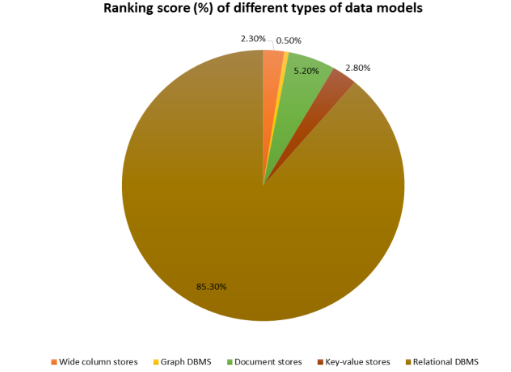
\includegraphics[height=7cm, width=9cm]{../../../images/rank.png}
	\caption{Ranking score of different types of data models (Source: \cite{DBLP:journals/corr/Sharma15b})}
\end{figure}


\subsubsection{Security}\mbox{}

\noindent Currently under active development,
NoSQL databases are generally subject to a fairly long list of security issues \cite{deka2014handbook} such as weak password storage, lack of encryption support for the data files, weak authentication both between client and the servers, data at rest is unencrypted, etc.

\[\]

\section{Conclusions}

Nowadays, the exponential usage of digital devices and massive data generation that comes after post both great opportunities and also unprecedented challenges to all data managing enterprises, startups, institution as well as data scientists and engineers.
The demand to scale out in order to store and process the accumulating data is a urgent problem as business expands and the client pool enlarges. That's when NoSQL comes into play. This paper gives a precise introduction of the  features (Availability, Scalability and Consistency) of NoSQL DBMS and provides comparisons among some of the most widely used NoSQL databases from their architectures, data models and suitable applications and scenarios. The classification (key-value store, column-oriented store, document-oriented store and graph-based store) and the most prominent representatives of each are also discussed. The benefits and drawbacks illustrated are aimed to help both academic and industrial users to have a more thorough understanding of NoSQL databases before deciding which one or ones to use for their own tasks. NoSQL as a promising alternative for the conventional relational database system, presents its unparalleled advantages especially when manipulating amount of data up to petabytes or terabytes and unstructured sparse data, which makes the comparison and evaluation among popular NoSQL database systems in analyzing big data a potential subject in future work that is worth further exploration. 

\[\]
